\documentclass[12pt,a4paper]{report}
%Encabezado segun reglas de trabajo final

% Paquetes usados
\usepackage[latin1]{inputenc}
\usepackage[spanish]{babel}
\usepackage{fancyhdr}
%\usepackage{fullpage}
\usepackage{graphicx}
\usepackage{psfig}
\usepackage{subfigure}
\usepackage{color}
\usepackage{fancybox}
\usepackage{graphics}
\usepackage{amssymb}
\usepackage{hyperref}
\usepackage[centerlast,small,bf]{caption2}
\usepackage{template}

% Formateador de  portada
\newcommand{\THESISNAMEA}{Impresora Braille - Implementaci\'on libre }
\newcommand{\THESISAUTHORA}{\hspace*{1in}Rosales Victor Hugo\hspace*{1.2in}787774}
\newcommand{\THESISAUTHORB}{\hspace*{1in}German Horacio Sanguinetti\hspace*{1.2in}977969}
\newcommand{\THESISDATE}{Diciembre de 2008}
\newcommand{\THESISYEAR}{2009}
\newcommand{\THESISSINODALA}{Ing. John Coppens}
%-----------------------------------------------------------------------------------------

\title{\THESISNAMEA}
\date{\THESISDATE}

% No se que hace esto, por las dudas lo saque.
%\setcaptionwidth{13cm}

\psfigurepath{./img/}

% ----------------------------------------------------------------------------
\begin{document}

%------------------------------------------------------------------------------------------
% Portada principal

\sloppy
%\newpage
\thispagestyle{empty}
%\vspace*{-0.5in}
\begin{center}
%\hspace*{-0.6in}
{\bf \mbox{Universidad Cat\'olica de C\'ordoba}}\\
%{\bf CAMPUS ???? } \\
%\vspace*{0.15cm}
%\hspace*{-0.1in}

%\vspace*{0.7in}
{\bf TRABAJO FINAL} \\
%\vspace*{0.7in}
%{\bf VISION COMPUTACIONAL}\\
%\vspace*{0.4in}
{\bf \THESISSINODALA} \\
%\vspace*{1in}

\begin{large}{\bf \THESISNAMEA}\end{large} \\
\end{center}
%\vspace*{0.4in}
%\vspace*{0.4in}
{\bf \THESISAUTHORA} \\
{\bf \THESISAUTHORB} \\
%\vspace*{0.5in}

%\begin{center}
%\begin{figure}[h]
%\centerline{\psfig{file=example.eps,width=3in}}
%\end{figure}
%\end{center}

\begin{center}
%\vspace*{0.5in}
{\bf C\'ordoba, Argentina., \THESISDATE}
\end{center}


\sloppy
\newpage
\thispagestyle{empty}

\begin{center}
\section*{Agredecimientos}
... a todos aquellos que hicieron, hacen y har\'an que mi vida valga la pena
...
\end{center}

% -----------------------------------------
\tableofcontents  %% Genera indice general.
% -----------------------------------------

\chapter{Pr\'ologo} %%%%%%%%%%%%%%%%%%%%%%%%%%%%%%%%%%%%%%%%%%%%%%%%%%%%%%%%%%%
%%%%%%%%%%%%%%%%%%%%%%%%%%%%%%%%%%%%%%%%%%%%%%%%%%%%%%%%%%%%%%%%%%%%%%%%%%%%%%%
% Prólogo, donde se definan sus alcances, propósitos y objetivos.
% Requerido por reglamento de trabajo final 

Durante el transcurso del trabajo se describe el desarrollo e implementaci\'on
de la parte electr\'onica de una impresora braille. El objetivo final del
mismo es proveer una posible soluci\'on de bajo costo, tanto de producc\'ion
como de armado. Para ello, se estudiar\'an y analizar\'an todas aquellas
alternativas disponibles que puedan satisfacer los requerimientos
planteados.\\

La principal premisa con que se aborda el desarrollo de este trabajo es que
mediante soluciones b\'asicas y simples, es posible concretar dise\~nos
robustos y funcionales, siempre y cuando se hayan elegido las herramientas y
condiciones correctas. Para lograr esto, gran parte del trabajo se centra en
investigar alternativas de desarrollo no convencionales en la industria
electr\'onica.

% Prólogo, donde se definan sus alcances, propósitos y objetivos.



% Segun reglamento de trabajo final
% Desarrollo, en esta parte se deben incorporar todos los conocimientos 
% Ingenierilesque permitan superar los problemas planteados.
% No necesariamente se deben llegar a resultados positivos, puede suceder que
% se obtengan resultados negativos y son tan válidos como los anteriores, no
% olvidar que la idea del T. F. es como el primer trabajo profesional.
% En este punto es importante hacer intervenir la mayor cantidad de materias
% que se han cursado, porque fundamentalmente estamos hablando de un trabajo
% integrador.

%---------------------------------------------------------------------------
% Cada capitulo debe ser un archivo separado para mejor mantenimiento.
% Ademas cada capitulo debe tener
% \chapter{title}
%
%	- Prologo del capitulo sin ningun formato especial(?)
%	- Secciones....
%---------------------------------------------------------------------------
% Requerido por reglamento de trabajo final 
\chapter{Resumen}

% Resumen, donde se describe brevemente el trabajo realizado-
% Una idea inicial de resumen es la que se escribe a continuacion
% se pueden repetir lo incluido en diagnostico y objetivos siempre que no tenga
% una extension considerable que sobrepase la caracteristica de resumen

El siguiente trabajo describe los pasos para construir un dispositivo simple
para la impresion de texto Braille, mediante la utilizacion de SL durante todas
las etapas del proyecto. El dispositivo tiene las funcionalidades esenciales de
una impresora Braille, suficientes para lograr el estampado de los puntos del
codigo sobre el papel Braille. El trabajo se focaliza sobre la aplicacion de
herramientas libres en la obtencion de un elemento que hereda estas
caracteristicas, contemplado en el tipo de licencia utilizado % para este
%trabajo. 
Se hara refrencia a la impresora Braille como embosser en el transcurso de este
trabajo.
% embosser se traduciria a estampadora o gofradora, dispositivo de gofrado

%

% Pueden agregarse secciones si es necesario
%\section{Ejemplo} 

% Uno de los capitulos iniciales del cuerpo del trabajo, contiene una
% introduccion del capitulo y el marco teorico de los diferentes enfoques
% posibles como formas de implementar el trabajo.
\chapter{Propuestas iniciales}
% Comentario de este capitulo 
\section{Introduccion} 
% Explicar que son los puntos que se mencionan a continuacion 
\section {Enfoque estilo industrial}
% modificar el titulo anterior en caso de no ser apropiado, puede encontrarse
% una referencia bibliografica para respaldar la eleccion (conveniente pero no
% excluyente)
Este enfoque de proyecto se basa en generar un producto para ser inyectado en
el mercado de las impresoras braille, mediante el dise\~no de todo el esquema de
produccion, la determinacion de los recursos que intervienen como factores de
la produccion y del ciclo de vida del producto. Corresponde a un esquema clasico
y convencional que consiste en la explotacion de materia prima, recursos
humanos, infraesctructura y soporte financiero para establecer un producto
industrial. El factor economico interviene de forma imperativa en este
paradigma de fabricacion y la motivacion es enteramente lucrativa. 
Generalmente estos aspectos son los que definen la economia de escala, que
junto con los factores de la produccion definen la rentabilidad.
El dise\~no se inicia con un estudio de la demanda y la inclusion del producto en
el mercado existente de impresoras (incluyendo los circuitos de distribucion, 
comercializacion y servicios), hasta llegar al consumidor final.
El beneficio se define en funcion del precio (valor agregado del producto
final) y de los costos que intervienen en la cadena de produccion. 
El fin de este modelo es la comercializacion, sustentado unicamente por la
competencia en el mercado. 
Esta caracteristica conduce a la complejidad no necesaria del dispositivo para
hacerla competente dentro del mercado. Por ejemplo, incluir una caracteristica
de compatibilidad con un producto cualquiera ("Bista compatible" por ejemplo) 
que tiene unico fin de aumentar las ventas, incidiendo en los consumidores al
manipular sus desiciones de consumo (competencia agresiva).
A su vez quedan implicitos altos costos por solo uso de marca y pago de 
licencias, y sin impacto en la calidad como producto.
Como consecuencia de adoptar este modelo de trabajo, los factores que conducen
a elevado precio final y la falta (o lentitud) de subsidios nacionales
para financiar el precio pueden llegar a injustificar completamente la 
realizacion de este proyecto por no ser rentable (y de hecho asi sucede en
Argentina, no existe una sola fabrica de impresoras Braille).
% Respaldar el parentesis anterior con con la referencia de la investigacion
% realizada 
Ademas no soluciona el problema estructural ya que el alcance de estas
impresoras seria para sectores sociales de alto poder adquisitivo.
\section {Enfoque estilo investigacion financiada}
% nuevamente modificar el titulo anterior si no es apropiado, puede encontrarse
% una referencia bibliografica para respaldar la eleccion (conveniente pero no
% excluyente)
Este enfoque se centraliza en adoptar una metologia de trabajo bajo el concepto
de investigacion clasica, avalada por una institucion, estado  o empresa como
inversion en materia economica. Los costos son mas flexibles, pero pueden ser
mas limitados segun la escala (al tratarse de trabajos por producto o por
prototipo, la financiacion se establece en base a los resultados que influiran
en la inversion y no tanto en la necesidad inmediata).
Si bien hereda caracteristicas del modelo industrial (por ejemplo la
competencia aunque en este caso menos agresiva), la sustentbilidad del modelo
esta establecida por el valor que la inversion resulta y se traduce en
beneficio economico a largo plazo (generalmente conocida como I+D)
lo que en definitiva define en este caso el valor agregado. Los costos
nuevamnete aplican a recursos, patentes intelectuales, licenciamiento
propietario y uso de marcas.
El modelo apunta a desarrollar un prototipo que resuelva una necesidad 
haciendo uso de los recursos establecidos por el organismo que financia dicho
producto. Tampoco existe libertad en la eleccion de las herramientas mas
convenientes o una conveniencia tecnica determinada (generalmente se adoptan
elementos de uso masivo y nunca se pregunta por que) y como resultado 
el proyecto terminado hereda estos atributos restrictivos que terminan
impactando en la libre eleccion de recursos y tecnicas optimas de
implementacion. 
\section {Enfoque alternativo}
% nuevamente modificar el titulo anterior si no es apropiado, puede encontrarse
% una referencia bibliografica para respaldar la eleccion (conveniente pero no
% excluyente)
%
% Este parrafo es el fundamental y debe ser redactado cuidadosamente se\~nalando
% las caracteristicas esenciales de un desarrollo autosustentable, el valor
% agregado es el beneficio social y principalmente este enfoque no trabaja
% sobre un mecanismo de competencia sino de cooperatividad, que le da la
% sustentabilidad suficiente para evolucionar.
% observar fundamentando este punto la caracteristica comunitaria del SL y el
% fenomeno de formacion de comunidades naturalmente
% tambbien se\~nalar que implica un riesgo por ser un enfoque diferente y
% original (lo no convencional despierta miedo) y el riesgo es el rechazo por 
% 
\section{Enfoque utilizado} 
El trabajo fue realizado siguiendo las ideas establecidas en el ultimo enfoque
descrito, que se justifica por las siguientes razones:
% enumerar y dar razones de por que seguir el camino no convencional

% capitulo que contiene el desarrollo tecnico del disposotivo (hardware y
% software), convencionalmente fue decidido iniciar por el dise\~no de hardware
% y luego continuar con la programacion del hardware (software embebido p
% firmware) y finalmente el programa que se ejecuta en la PC (software)

\chapter{Propuesta T\'ecnica}
% Comentario de este capitulo 

\section{Introduccion} 

% Breve introduccion para mencionar como se van a desarollar los temas 
% incluidos en este capitulo, que se propone obtener y basicamente presentar
% los tres bloques mas importantes: harware, firmware y software.
% la organizacion no es definitiva y puede cambiar su orden, se propone un
% draft inicial.
% TBD: Verificar la redaccion y agregarle formalismo tecnico, reorganizar
% revisi\'on por parrafos pendientes para volver a redactar las ideas escritas.

En este capitulo se explica a continuacion el procedimiento t\'ecnico
desarrollado para construir una impactadora de codigo braille.
Como primera propuesta, se comienza en investigar y adaptar una impresora a
matriz de puntos a modo de prototipo para lograr imprimir codigo sobre papel
comun, sin alterar demasiado su funcionamiento regular y mantieniendo
preferentemente los elementos actuadores.
Se realizan algunas adaptaciones mecanicas y electricas, y mediante un sencillo
programa se traduce un texto de sample enviando el conjunto de caracteres
codificados para actuar sobre las funciones de la impresora.
Ademas se presenta el dise~no de la electr\'onica de control para el
accionamiento de los elementos meacnicos, utilizando el microcontrolador
PIC18F4550. Este procesador incorpora un modulo USB y el funcionamiento del SIE
ser]'a explicado en detalle.
Tambi\'en se incluir\'an las simulaciones y mediciones necesarias para la
calibraci\'on y puesta a punto de los dispositivos mecanicos (velocidad de los
motores electricos, niveles de corriente y carga, tiempo de trabajo necesario
para el percutor imprima los puntos y regrese a su posici\'on de origen, etc).
% ...
El percutor consiste en un sistema mecanico sencillo de un unico elemento
impactador que ser\'a accionado mediante una corriente electrica. 
No se profundizar\'an los detalles del dise\~n o mecanico ya que sale fuera
del alcance de este trabajo, y dada su prioridad sera el ultimo elemento a
construir.
Un circuito de control adicional maneja el percutor en la forma que adecuada,
en la programaci\'on del microcontrolador se realizan los cambios necesarios 
para modificar el pulso (o pulsos) que se necesiten para enviar la se\~nal de 
activacion a los diferentes tipos de solenoides.
Los motores ser\'an abordados de forma independiente, para controlar el
movimiento 
rotacional y transversal, de modo de ubicar el carro en el lugar de impacto. 
Una calibracion adicional sera necesaria para ajustar la velocidad
% que sera resuelta con un circuito de prueba especialmente contruido para este
% fin (obtener los parametros de funcionamiento mecanico)
% ...
% ????

\section {Dise\~no electr\'onico (Hardware)}

% modificar el titulo anterior en caso de no ser apropiado, puede encontrarse
% una referencia bibliografica para respaldar la eleccion (conveniente pero no
% excluyente)
% ------------------------------------------------------------------------
%
% Contenido principal de la seccion
%
% ------------------------------------------------------------------------
% \subsection{Firmware}
% Respaldar el parentesis anterior con con la referencia de la investigacion
% realizada 
%
\section {Dise\~no l\'ogico (Software)}

% nuevamente modificar el titulo anterior si no es apropiado, puede encontrarse
% una referencia bibliografica para respaldar la eleccion (conveniente pero no
% excluyente)
% ------------------------------------------------------------------------
%
% Contenido principal de la seccion
%
% ------------------------------------------------------------------------
%
%\section {Nombre_seccion}
%
% ------------------------------------------------------------------------
%
% Contenido principal de la seccion
%
% ------------------------------------------------------------------------
% 

% El objetivo de este capitulo es presentar a grandes rasgos el dispositivo 
% y luego sus detalles. Sus caracteristicas  mas importantes, explicar el 
% funcionamiento, alternativas, diagramas, comparaciones, ventajas y desventajas
% de cada opcion, como presentar tambien los detalles pertinentes, los factores
% principales y prioritarios.
\chapter{El dispositivo}
% Comentario de este capitulo 
\section{Introduccion} 
% Breve introduccion para presentar el dispositivo visto como prototipo que
% tiene que cumplir determinada funcion, planteando los requerimientos y
% ampliando en detalles gradualmente a medida que se avanza en la lectura
% el enfoque tiende a ser teorico antes de abordar cualqueir conclusi�n parcial
% pr�ctica
La impresora Braille o embosser (estampadora) es un dispositivo que realiza un
estampado en relieve de arreglo de puntos sobre un papel ductil, de manera 
autom�tica (es decir no-manual).
% incluir un diagrama en bloques simplificado del sistema completo aqui mismo.
\section {El sistema Braille}
% Draft inicial de esta seccion. Ampliarla de acuerdo a la relevancia e incluir
% figuras y gr�ficos
El sistema Braille es un m�todo utilizado por personas ciegas para leer y 
escribir. Fue ideado en 1821 por el franc�s Louis Braille
Se basa en un m�todo de comunicaci�n desarrollado y perfeccionado por Charles 
Barbier en respuesta a la demanda de Napole�n de un c�digo que los soldados 
pudieran usar para comunicarse en silencio y sin luz en la noche y se lo llam� 
Night writing. El sistema de Barbier era demasiado complejo para los soldados de 
aprender, y fue rechazada por los militares. En 1821 visit� el Instituto Nacional 
para Ciegos, en Par�s, Francia, donde conoci� a Louis Braille. Braille identificado 
el mayor defecto de c�digo, que es que el dedo de la mano humana no puede abarcar 
todo el s�mbolo sin moverse, y as� no puede pasar r�pidamente de un s�mbolo a otro.
Su modificaci�n fue utilizar una celda de 6 puntos - el sistema Braille - que 
revolucion� la comunicaci�n escrita de los ciegos.
Cada c�lula (o celda) braille o car�cter se compone de seis posiciones de puntos,
dispuestos en un rect�ngulo que contiene dos columnas de tres puntos cada uno. Un
punto puede ser colocado en alguna de las seis posiciones para formar sesenta y 
cuatro (2^6) permutaciones, incluido el arreglo de puntos que no se coloca. Una 
permutaci�n puede ser descrita nombrando las posiciones en que se disponen los 
puntos: Las posiciones est�n universalmente numerados de 1 a 3, de arriba a abajo, 
a la izquierda, y 4 a 6, de arriba a abajo, a la derecha. 
%Por ejemplo, puntos 1-3-4 describir�a una celda con tres puntos planteados, en la parte superior e inferior de la columna de la izquierda y en la parte superior de la columna de la derecha, es decir, la letra m. 
Las l�neas horizontales de texto en Braille est�n separados por un espacio a
fin de que los puntos de una l�nea puede ser diferenciada de la de texto en 
braille por encima y por debajo. La puntuacion est� representada por su propio 
conjunto de caracteres �nico.
% incluir figuras para facilitar la explicacion

%\section {Nueva_seccion}
% nuevamente modificar el titulo anterior si no es apropiado, puede encontrarse
% una referencia bibliografica para respaldar la eleccion (conveniente pero no
% excluyente)
%
% 
% 

\section{Software Libre}

El Software Libre, es aquel que le asegura cuatro libertades b\'asicas al
usuario. La libertad de usa el programa, de estudiar su funcionamiento, de
compartirlo y la libertad de mejorarlo y distribuirlo.

\subsection{Historia}
El concepto de Software Libre (Free Software) comienza a gestarse en la 
d\'ecada del 60/70. En ese entonces el software no era considerado un
producto, sino m\'as bien un a\~nadido que formaba parte del hardware. Por esta
raz\'on las personas que trabajaban con software compart\'ian sus c\'odigos
fuentes libremente. A finales de los 70, las compa\~n\'ias de software
comenzaron a implementar licencias a sus programas con ciertas restricciones. 
Surg\'ia entonces la necesidad de tener un sistema operativo libre donde
correr aplicaciones libres.


\subsection{GNU}
En 1984, un estudiante del Instituto de Tecnolog\'ia de Massachusetts
(Massachusetts Institute of Technology - M.I.T), llamado Richard Stallman, 
comenz\'o a desarrollar el proyecto G.N.U (GNU's not UNIX).
\'Este, pretendia ser un reemplazo libre de los sistemas propietarios que 
estaban surgiendo en aquella \'epoca.
Sus motivos\footnote{V\'ease ''Manifiesto GNU'' - 
http://www.gnu.org/gnu/manifesto.es.html} eran diversos, pero principalmente 
cre\'ia que era necesario desarrollar un entorno l\'ibre para las personas.
Para llevar acabo su proyecto se bas\'o en UNIX, un sistema operativo 
portable multiusuario y multitarea. Junto con la Colecci\'on de Compiladores
GNU (GCC)\footnote{Previamente llamado -GNU C Compiler- puesto que solo
compilaba codigo C. Versiones m\'as recientes soporta varios leguajes. V\'ease
- http://gcc.gnu.org}, un editor de texto y todo un stack de software,
comenz\'o a idear el proyecto GNU.

\subsection{GNU/Linux}
El proyecto GNU tomaba forma pero le faltaba un componente muy importante; el
kernel. 
En 1991, un estudiante finland\'es llamado Linus Torvalds, liber\'o un kernel
basado en UNIX, que luego pasar\'ia a formar parte de lo que hoy se conoce como
GNU/Linux.
GNU/Linux es un sistema operativo completo con un stack de software que
satisface la mayoria de las necesidades de un usuario m\'as un potente kernel
mutiplataforma.\
Lo que hace a GNU/Linux (y a la mayoria de los programas libres) versatiles,
robustos y estables, es que se basan en estandares abiertos y libres, como lo
son \emph{SUS}\footnote{Single Unix Specification - V\'ease -
\url{http://en.wikipedia.org/wiki/Single_UNIX_Specification}},
\emph{POSIX}\footnote{V\'ease - \url{http://en.wikipedia.org/wiki/Posix}} o
\emph{IEEE}\footnote{V\'ease - \url{http://www.ieee.org}}.

\subsection{Concepto de Software Libre}
Luego del proyecto GNU, Richard Stallman fund\'o la Fundaci\'on para el 
Software Libre (Free Software Foundation)
\footnote{V\'ease - http://www.fsf.org} quien se encarga (entre otras cosas) de
mantener la definici\'on del concepto\footnote{V\'ease -
http://www.fsf.org/licensing/essays/free-sw.html} de Software Libre.

\begin{quote}
``Free software'' is a matter of liberty, not price. 
To understand the concept, you should think of ``free'' as in ``free speech,
'' not as in ``free beer.''
\end{quote}

% Poner en cursiva o algo para resaltar que es una traduccion
El Software Libre es una cuesti\'on de libertad no de precio\footnote{\'Esta
aclaraci\'on surge debido a que en ingl\'es, \emph{free} significa tanto
\emph{libre} como \emph{gratis}.}. Para entender el concepto debe pensar libre
(\emph{free}) como en libre discurso no como cerveza gratis.\\

Para que un programa sea Software Libre, debe garantizarle cuatro libertades
b\'asicas al usuario:

\begin{itemize}
\item[Libertad 0:] Libertad de ejecutar el programa con cualuier prop\'osito
\item[Libertad 1:] Libertad de estudiar como funciona el programa y de
adaptarlo
a tus necesidades. \emph{Acceso al codigo fuente es un pre-condici\'on para
\'esto}
\item[Libertad 2:] Libertad de redistribuir copias del mismo para poder ayudar
a tu vecino.
\item[Libertad 3:] Libertad de mejorar el programa y pulicar los cambios para
que toda la comunidad se beneficie de ellos. \emph{Acceso al codigo fuente es 
un pre-condici\'on para \'esto}
\end{itemize}


\subsection{El Software Libre en la ingenieria} 
% No me gusta como suena el titulo este
Existen en la actualidad tecnologias o herramientas libres para lidiar con la
mayoria de los problemas de la ingenieria. Pero que, debido a su propia
naturaleza libre u \emph{open source}, carecen de publicidad suficiente como
para competir con sus alternativas \emph{propietarias}. \\

No obstante su condicion libre, la mayoria de estas tecnologias estan a la
altura de sus pares \emph{propietarios}. Tanto es asi que existen empresas que
se dedican exclusivamente a este tipo de tecnologias\footnote{Vease -
http://www.redhat.com/ - http://code.google.com/opensource/}, y otras grandes
empresas como Intel\footnote{Vease - http://software.intel.com/sites/oss/},
IBM\footnote{Vease - http://www.ibm.com/developerworks/opensource/} y
Motorola\footnote{Vease - https://opensource.motorola.com/}, trabajan
activamente en proyectos libres.\\

\chapter{Anexo: el mercado del software}
% Esta copiado e inspirado del Periodico de la Universidad Nacional de Cordoba,
% nota de tapa de la fecha - Domingo 14 de Diciembre 2008 - Numero 46
% No olvidar agregar la referencia bibliografica correspondiente.
% La UNC invita a la difusi�n del art�culo, sirve para respaldar y refozar 
% el capitulo de software libre por eso est� agregado como anexo. 
% Tambien queda pendiente hacer el formateo de lineas y correcion de
% internacionalizacion de acentros y carateres especiales
\section{Software libre y el mercado del software}
El dominio exclusivo del mercado del software en manos de una sola empresa ha
impuesto un v�nculo restrictivo y privativo de la tecnolog�a para con sus
usuarios. Para la UNC, se hace necesario y urgente problematizar esta situaci�n
y modificarla como condici�n ineludible de una democracia que garantice los
derechos y libertades de los ciudadanos. 
El sistema operativo y los programas que mayoritariamente se utilizan en las
computadoras personales integran lo que se conoce como Software Propietario,
cuyas dos principales caracter�sticas son: que no permite el acceso a su c�digo
fuente -estructura de funcionamiento-, constituyendo un producto cerrado donde
nadie puede conocer las acciones que ejecuta el programa, tampoco modificarlo o
corregir sus errores; y que su distribuci�n se realiza en base al pago de
licencias, la autorizaci�n para su uso. Por estas caracter�sticas se lo denomina
tambi�n Software Privativo, ya que restringe libertades de los usuarios, tanto
en la utilizaci�n de los programas como en la posibilidad de disponer de ellos.
Como comprar un auto sin capot, donde cualquier ruido, falla o modificaci�n,
ser�a imposible de resolver para due�o o mec�nico algudno. Un veh�culo sellado
donde toda correcci�n o mejora s�lo es posible a trav�s de un segundo producto,
que por supuesto vendr� a sustituir al anterior obligando a una nueva compra. 
Este tipo de reglas de juego incorporadas  y asumidas  socialmente como el modo
natural de v�nculo con la tecnolog�a no tiene nada de razonable, sin embargo es
el modelo que impulsan las empresas que dominan el mercado del software. En
primer lugar, el concepto de licencia implica que uno no est� comprando el
producto y la posibilidad de disponer de �l, sino que pada una autorizaci�n para
usarlo. Adem�s estas empresas imponen una pol�ticadde incompatibilidad en la que
sus programas trabajan con formatos propios (no esd�ndares) que no pueden ser
abiertos por programas similares ni reconocen los archivos de otros. Pero
tambi�n, incompatibilidades dentro de la misma marca ya que la versi�n anterior
no reconoce archivos de la versi�n nueva, obligando al usuario a la renovaci�n
permanente.
El poder�o de una empresa o marca se hace  tangible cuando sus l�gicas,
condiciones particulares de funcionamiento y, sobre todo, defectos se imponen
como los modos naturales de entender la realidad. As� "se cay� el sistema" ha
pasado de ser una frase incomprensible y odiosa a excusa v�lida y recurrente. La
naturalidad con que las personas aceptan este argumento es un triunfo del modelo
del software privativo. Las fallas de un programa se imponen y est�n modificando
los tiempos, necesidades y posibilidades de los sujetos.
GrULIC define Software Libre como aquel que garantiza a sus usuarios "la
libertad para ejecutar, copiar, distribuir, estudiar, cambiar y mejorar el
software". Y enumera cuatro libertades fundamentales: la de usar el programa con
cualquier prop�sito; la de estudiar como funciona y adaptarlo a las necesidades
de cada uno (el acceso al c�digo fuente es una condici�n para esto); la de
distribuir copias; y la de mejorar el programa y hacer p�blicas las mejoras, de
modo que toda la comunidad se beneficie.
Existe una diferencia sustancial en el tipo de v�nculos que se establecen entre
tecnolog�a y usuario. Mientras esta concepci�n se define por las libertades que
otorga y garantiza, el Software Propietario se caracteriza por las restricciones
y obligaciones que demanda.
El monopolio de hecho que ostenta la marca l�der ha redundado en la imposici�n
de sus formatos. Frente a esto, dada su flexibilidad y el aporte de sus propios
usuarios, el software libre ha logrado adaptarse a esta situaci�n. Open Office,
procesador de texto de software libre, permite reconocer archivos de Word 2007
(.docx), un formato incompatible con la versi�n 2003 del mismo programa. La
calidad de estos productos tiene que ver con una cuesti�n f�sica que viene de su
estructura de funcionamiento y con una cuesti�n conceptual respecto de la
construcci�n del conocimiento. Se trata de un mont�n de personas aportando al
mismo producto; la multiplicidad de ideas lo enriquece en adaptabilidad y
amplitud porque cada usuario aporta a una necesidad concreta; y la libertad de
distribuci�n y reproducci�n nos pone a todos en igualdad de condiciones para
aprovechar esos avances.La principal forma de negar la libertad es la que impone
la noci�n de que s�lo existe una opci�n posible. 
La opci�n de software propietario implica costos altos de licenciamiento m�s un
monto adicional por documento ingresado al sistema; pero sobre todo, en su
condici�n de sistema cerrado, este programa no trabaja con formatos est�ndares
lo que provoca una dependencia estrecha con una empresa y de cualquiera de sus
vicisitudes ya que ser�a la �nica con posibilidades de decodificar lo que
ingrese a su sistema.
El principal ingreso de las empresas de software propietario proviene del cobro
de las licencias por el uso de sus productos. Sin embargo, en los pa�ses en v�as
de desarrollo, la principal estrategia ha sido la de permitir, o por lo menos
dejar pasar, la reproducci�n y distribuci�n indiscriminada entre los usuarios
individuales y de peque�a escala.
La facilidad en la obtenci�n de copias hace perder de vista la idea de que las
personas deben pagar para utilizar dichos programas, mientras que la
multiplicaci�n de usuarios funciona como una barrera de contenci�n a la
posibilidad de implementar o siquiera sugerir sistemas alternativos. Si uno
tuviera que pagar por el sistema operativo de su computadora los \$500 que
cuesta la licencia, entonces ser�a m�s exigente con su funcionamiento. Aunque en
realidad, cada vez que instalamos Software Propietario, estamos haciendo un
aporte a estas empresas porque cuando hacemos circular sus archivos tambi�n
estamos forzando al mercado a inclinarse en esa direcci�n.
La utilizaci�n de software libre en este caso nos permite compartir los
esfuerzos de aplicaci�n para reducir costos y adem�s, todos los avances que se
logran incorporar al programa pueden ser reutilizados.
Cuando se tiene acceso al c�digo fuente, hay independencia del proveedor en lo
econ�mico y en el tiempo, no hay riesgos de que la empresa propietaria cierre o
sea comprada por otra que discontin�e sus productos.
Hay varias razones de peso para definir la importancia del uso de Software Libre
en el Sector P�blico, estas razones son tanto pol�ticas como econ�micas y de
seguridad. Pero hay algo que debemos mencionar previamente, y es que el uso de
Software Libre en la Administraci�n P�blica es un imperativo si el Estado
pretende cumplir con obligaciones b�sicas que tiene frente a sus ciudadanos. Es
decir, no s�lo se trata de ventajas, sino que se trata de una situaci�n donde el
Estado s�lo puede cumplir parte de su misi�n si lo hace con software libre.
El Estado administra datos que no le pertenecen, datos que nos pertenecen a
nosotros como ciudadanos y que estamos obligados a entregarle por diferentes
razones. Desde declaraciones de bienes y ganancias hasta informaci�n filiatoria,
domicilio, estado de salud en muchos casos. Toda esta informaci�n que administra
no le pertenece. Por lo tanto, no puede hacer lo que se le d� la gana con ella,
sino que debe respetar algunos principios esenciales de perennidad de los datos
(que estos datos est�n accesibles dentro de 100 a�os), que estos datos sean
accedidos por quienes corresponde y nadie m�s, que ning�n tercero tenga
injerencia sobre el control de estos datos ni pueda decidir que en alg�n momento
dejen de estar accesibles a quien corresponda. A su vez, debe garantizar la
seguridad de estos datos y la confidencialidad.
El Estado no es un usuario de software cualquiera que puede evaluar los riesgos
y tomar una decisi�n arriesgada en funci�n de modas, gustos o costos, porque sus
responsabilidades son mayores.
Estas garant�as de perennidad, accesibilidad por quien debe acceder y nadie m�s
y seguridad s�lo se logran si el Estado tiene a su vez control total sobre los
programas que usa. No ser�a l�gico esperar que desarrolle software propio para
toda su gesti�n, pero tampoco es l�gico que utilice software que no puede
controlar de ninguna manera. El Software Libre le brinda el justo equilibrio de
tener programas desarrollados, probados y en permanente mejora sin tener que
resignar el control de la gesti�n inform�tica en manos de ninguna compa��a
privada en particular.
Por otra parte, la implementaci�n de pol�ticas p�blicas muchas veces se realiza
a trav�s de sistemas inform�ticos. Usar software que no es auditable en estos
casos vulnera el principio de transparencia en los actos de gobierno.
Por �ltimo, el mejor argumento tiene que ver con la condici�n fundante de la
universidad tiene que y debe ser el espacio para producir conocimiento p�blico
que est� a disposici�n y al servicio de la comunidad: Generar ideas y saberes
para que otros puedan construir a partir de ello. Adem�s as� como se difunde lo
que se produce, tambi�n se puede disponer de lo que otros han generado. Ese
proceso es infinitamente m�s rico porque siempre habr� en circulaci�n m�s ideas
de lo que se puedan generar por cuenta propia. La tecnolog�a en s� misma no
tiene entidad ni intenci�n, pero tal caracter�stica no significa que su
incorporaci�n sea inocua o as�ptica, por eso es fundamental reflexionar respecto
de las posibilidades, oportunidades, restricciones y libertades que le aporta o
le quita a cada usuario y a toda la comunidad. Con diferentes grados de
implicancia y responsabilidades tanto en �mbitos p�blicos, como privados y
masivos como �ntimos, la elecci�n de una tecnolog�a, no puede librarse a la
inercia u omisi�n, porque all� tambi�n se ponen en juego las condiciones para
una mejor y m�s profunda democracia.
%***End***


\chapter{USB}
El \emph{Universal Serial Bus}(USB\footnote{V\'ease - http://www.usb.org}) es
un bus serial ent\'andar que hace de interfaz entre un dispositivo y una
computadora.
Dicha estandarizaci\'on es llevada acabo por el \emph{F\'orum de
Implementadores de USB} (USB Implementers Forum, USB-IF\footnote{V\'ease -
http://www.usb.org/about}). 
Actualmente el est\'andar se encuentra en su versi\'on 3.0\footnote{V\'ease -
http://www.usb.org/developers/docs/}, aunque la mayor\'ia de las
implementaciones comerciales solo soportan el ent\'andar \emph{2.0}.

%%%%%%%%%%%%%%%%%%%%%%%%%%%%%%%%%%%%%%%%%%%%%%%%%%%%%%%%%%%%%%%%%%%%%%%%%%%%%%
%%%%%%%%%%%%%%%%%%%%%%%%%%%%%%%%%%%%%%%%%%%%%%%%%%%%%%%%%%%%%%%%%%%%%%%%%%%%%%
\section{Historia}
%No me gusta como titulo 'historia' habria que pensar otra cosa

%%%%%%%%%%%%%%%%%%%%%%%%%%%%%%%%%%%%%%%%%%%%%%%%%%%%%%%%%%%%%%%%%%%%%%%%%%%%%%
%%%%%%%%%%%%%%%%%%%%%%%%%%%%%%%%%%%%%%%%%%%%%%%%%%%%%%%%%%%%%%%%%%%%%%%%%%%%%%
\section{Decripci\'on}
% Aca iria el funcionamiento del USB, difierenciado por \subsection{}
% Por ahora me estoy basando en la spec 2.0 oficial.
La especificaci\'on USB provee una serie de atributos con los cuales se pueden
implementar dispositivos seg\'un el precio/rendimiento deseado.

%%%%%%%%%%%%%%%%%%%%%%%%%%%%%%%%%%%%%%%%%%%%%%%%%%%%%%%%%%%%%%%%%%%%%%%%%%%%%%
\subsection{Caracter\'isticas}
Del amplio rango de caracter\'isticas definidas en el ent\'andar, es posible
agruparlas en ocho categor\'ias:
% Reescribir lo de arriba y agregar mas

\begin{itemize}
 \item Facilidad de uso para el usuario final
 \item Amplio rango de aplicaciones
 \item Ancho de banda is\'ocrono
 \item Flexibilidad
 \item Robustez
 \item Sinergia con la industria de la PC
 \item Implementaci\'on de bajo costo
 \item De arquitectura actualizable
\end{itemize}

La combinaci\'on de estas caracter\'isticas hacen a la versatilidad del
ent\'andar, ya que permiten implementar todo tipo de dispositivos seg\'un la
carga, versatilidad, eficiencia, precio, velocidad y dem\'as atributos que
puedan inferir en un diese\~no.\\

Para la veri\'on 2.0 de la epecificaci\'on, el protocolo soporta tres
velocidades de transimsi\'on como se muestra en la
tabla \ref{tab:velocidad_usb}.

\begin{table}[h]
\centering
% use packages: array,booktabs
\begin{tabular}{|c|c|}        \hline
High Speed & 480 Mbits/seg \\ \hline 
Full Speed & 12 Mbits/seg  \\ \hline
Low Speed & 1.5 Mbits/seg  \\ \hline
\end{tabular}
\caption{Velocidades de USB} 
\label{tab:velocidad_usb}
\end{table}

%%%%%%%%%%%%%%%%%%%%%%%%%%%%%%%%%%%%%%%%%%%%%%%%%%%%%%%%%%%%%%%%%%%%%%%%%%%%%%
\subsection{Arquitectura}

USB es un \emph{bus} cableado que soporta conexiones entre un \emph{host} y
gran rango de perif\'ericos. Dicho \emph{bus} permite la conexi\'on,
configuraci\'on, uso y desconexi\'on de un dispositivo mientras el \emph{host}
y dem\'as perif\'ericos est\'an en funcionamiento. \\

Un sistema USB se  define segun tres grandes \'areas:

\begin{itemize}
 \item Interconexi\'on USB
 \item Dispositivo USB
 \item \emph{Host} USB
\end{itemize}

%%%%%%%%%%%%%%%%%%%%%%%%%%%%%%%%%%%%%%%%%%%%%%%%%%%%%%%%%%%%%%%%%%%%%%%%%%%%%%
\subsubsection{Caracter\'isticas el\'ectricas}

USB usa cuatro cables para alimentaci\'on y se\~nal. La se\~nal viaja a travez
de un par trenzado diferencial y se encuentra codificada con Non Return to Zero
Inverted (NRZI). En la figura \ref{fig:electric_usb} se muestra un diagrama de
un cable
USB.

\begin{figure}
\centering
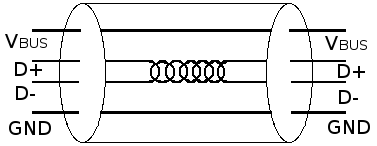
\includegraphics[scale=0.5]{./img/electric_usb.png}
\caption{Cable USB.}
\label{fig:electric_usb}
\end{figure}

Al ser un par diferencial, el host iterpreta un \emph{1} diferencial cuando D+
es 200 mV mayor que D- y un \emph{0} diferencial cuando D- es 200 mV mayor que
D+. 
Los dispositivos USB indican su velocidad mediante una resistencia de
\emph{pull-up} a 3.3 V. En el caso de un \emph{full speed device} se col\'oca
una resistencia de 1.5K en D+ a 3.3 V, y para \emph{low speed device} se coloca
una resistencia de 1.5K a 3.3 V, como se muestra en la figura
\ref{fig:electric_speed_usb}.
Algunos fabricantes sulen integrar estas resistencias de \emph{pull-up} dentro
de sus \emph{chips} para ser activadas mediante software.

\begin{figure}
\centering
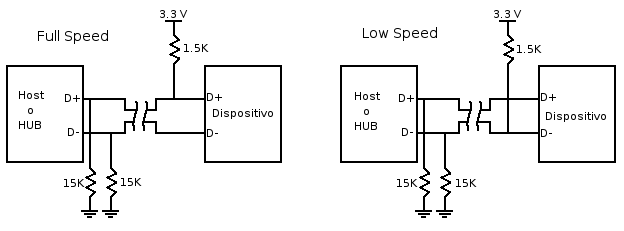
\includegraphics[scale=0.5]{./img/electric_speed_usb.png}
\caption{Velocidad USB.}
\label{fig:electric_speed_usb}
\end{figure}


%%%%%%%%%%%%%%%%%%%%%%%%%%%%%%%%%%%%%%%%%%%%%%%%%%%%%%%%%%%%%%%%%%%%%%%%%%%%%%
\subsection{Interconexi\'on USB}

La interconexi\'on USB define la manera en la que los dispositivos USB se
conectan entre si y con el \emph{host}. 

%%%%%%%%%%%%%%%%%%%%%%%%%%%%%%%%%%%%%%%%%%%%%%%%%%%%%%%%%%%%%%%%%%%%%%%%%%%%%%
\subsubsection{Topolog\'ia del bus}

USB usa una topolog\'ia de estrella por niveles. Un \emph{hub}\footnote{La
palabra \emph{hub} se traduce al castellano como \emph{centro}, pero su
traducci\'on no sera usada en este documento por cuestiones pr\'acticas.}
est\'a ubicado al centro de cada estrella. Las conexiones cableadas se dan
entre el \emph{host} y un \emph{hub} o funci\'on, entre \emph{hub} y
\emph{hub}, o entre un \emph{hub} y una funci\'on. \\

Debido a cuestiones de latencia, el n\'umero m\'aximo de niveles permitido es
siete, incluida la ra\'iz. La figura \ref{fig:usb_topology} muestra un esquema
de la topolog\'ia.

\begin{figure}
\centering
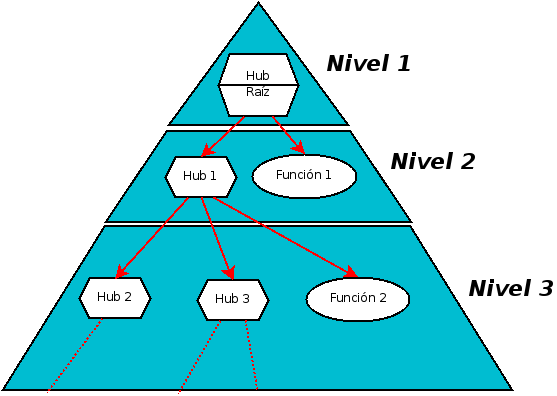
\includegraphics[scale=0.5]{./img/usb_topology.png}
\caption{Topolog\'ia del bus USB.}
\label{fig:usb_topology}
\end{figure}


%%%%%%%%%%%%%%%%%%%%%%%%%%%%%%%%%%%%%%%%%%%%%%%%%%%%%%%%%%%%%%%%%%%%%%%%%%%%%%
\subsection{\emph{Host} USB}

La especificaci\'on admite un solo \emph{Host} para un todo sistema USB. La
interf\'az USB del \emph{host}, se la denomina \emph{Host
Controller}\footnote{Al igual que con \emph{host}, esta palabra se mantedr\'a
en ingles.}. La implementaci\'on de un \emph{Host Controller} puede ser una
combinaci\'on de hardware, firmware o software. El \emph{hub} ra\'iz esta
integrado en el sistema \emph{host}, proveyendo puntos de acceso.
En la versi\'on 1.1 de la especificaci\'on, exixtian dos tipod de
controladores de \emph{hots}; \emph{Universal Host Controller Interface}
(UHCI)\footnote{Desarrolada por Intel} y \emph{Open Host Controller Interface}
(OHCI)\footnote{Desarrollada por Compaq, Microsoft y National Semiconductors}.
Luego con para le versi\'on 2.0 de la especificaci\'on de defini\'o un tercer
controlador; \emph{Enhanced Host Controller Interface} (EHCI)\footnote{Que
luego pasaria a convertirse en el estandar mas usado.}


%%%%%%%%%%%%%%%%%%%%%%%%%%%%%%%%%%%%%%%%%%%%%%%%%%%%%%%%%%%%%%%%%%%%%%%%%%%%%%
\subsection{Dispositivo USB}

Los dispositivos USB pueden ser dispositivos funcionales o bien \emph{hubs}.
En ambos casos deben ser capaces de entender el protocolo USB y responder a
peticiones estandares USB ademas de cumplir su funci\'on intr\'inseca. 

% Explicar --- UHCI, OHCI, EHCI
%\begin{Huge} TERMINAR!!! \end{Huge}


El protocolo USB define capas de abstracci\'on, cada cual con una funcionalidad
espec\'ifica. Normalmente los \emph{chips} manejan las capas mas bajas, para
abstraer al usuario de todo lo que ocurre en lo mas bajo del protocolo.\\

Una transacci\'on USB consiste de los siguientes paquetes:
\begin{itemize}
 \item Token (paquete cabecera)
 \item Data (opcional)
 \item Status (handshaking)
\end{itemize}

Los paquetes USB tienen ciertos campos comunes: 
\begin{itemize}
 \item Sync: Es un campo de sincronismo y todos los paquetes deben comenzar
con uno.
 \item PID: Es el identificador de paquete que informa el tipo de paquete que
es.
 \item ADDR: Es la direcci\'on a la cual esta asignado el paquete
 \item ENDP: Este campo de 4 bits permite direccionar hasta 16
\emph{endpoints}.
 \item CRC: Lleva la informaci\'on de un chequeo de redundancia c\'iclica de
los datos
 \item EOP: Este campo indica la finalizaci\'on del paquete.
\end{itemize}

%%%%%%%%%%%%%%%%%%%%%%%%%%%%%%%%%%%%%%%%%%%%%%%%%%%%%%%%%%%%%%%%%%%%%%%%%%%%%%
\subsubsection{Paquete \emph{Token}}
Los paquetes \emph{token} son usados para indicar el tipo de transacci\'on que
se realizar\'a. Existen tres tipos de paquetes \emph{token}:

\begin{itemize}
 \item IN - Informa al dispositivo USB que el host desea leer informaci\'on
 \item OUT - Inrofma al dispositivo USB que el host desea escribir
informaci\'on
 \item Setup - Es usado para comenzar transferencias de control
\end{itemize}

Un paquete \emph{token} esta formado por los siguientes campos mostrados en la
tabla \ref{tab:usb_token_fields}


\begin{table}[h]
\centering
% use packages: array,booktabs
\begin{tabular}{|c|c|c|c|c|c|} \hline
Sync & PID & ADDR & ENDP & CRC5 & EOP\\ \hline
\end{tabular}
\caption{Campos Token} 
\label{tab:usb_token_fields}
\end{table}


%%%%%%%%%%%%%%%%%%%%%%%%%%%%%%%%%%%%%%%%%%%%%%%%%%%%%%%%%%%%%%%%%%%%%%%%%%%%%%
\subsubsection{Paquete \emph{Data}}
Un paquete \emph{data} esta formado por los siguientes campos mostrados en la
tabla \ref{tab:usb_data_fields}

\begin{table}[h]
\centering
% use packages: array,booktabs
\begin{tabular}{|c|c|c|c|c|} \hline
Sync & PID & DATA & CRC16 & EOP\\ \hline
\end{tabular}
\caption{Campos Data} 
\label{tab:usb_data_fields}
\end{table}


%%%%%%%%%%%%%%%%%%%%%%%%%%%%%%%%%%%%%%%%%%%%%%%%%%%%%%%%%%%%%%%%%%%%%%%%%%%%%%
\subsubsection{Paquete \emph{Status}}
Los paquetes \emph{status} son usados para indicar el tipo de estado de la
transacci\'on. Existen tres tipos de paquetes \emph{status}:

\begin{itemize}
 \item ACK - Reconocimiento de que el paquete fue recibido.
 \item NAK - Avisa de que el dispositivo no puede recibir ni enviar datos.
 \item STALL - Significa que el dispositivo necesita la intevenci\'on del host.
\end{itemize}

Un paquete \emph{status} esta formado por los siguientes campos mostrados en la
tabla \ref{tab:usb_status_fields}.

\begin{table}[h]
\centering
% use packages: array,booktabs
\begin{tabular}{|c|c|c|} \hline
Sync & PID & EOP\\ \hline
\end{tabular}
\caption{Campos Status} 
\label{tab:usb_status_fields}
\end{table}


%%%%%%%%%%%%%%%%%%%%%%%%%%%%%%%%%%%%%%%%%%%%%%%%%%%%%%%%%%%%%%%%%%%%%%%%%%%%%%
%%%%%%%%%%%%%%%%%%%%%%%%%%%%%%%%%%%%%%%%%%%%%%%%%%%%%%%%%%%%%%%%%%%%%%%%%%%%%%
\section{Enpoints}
Un aspecto muy importante del estandar USB es la forma en la que se logra la
comunicaci\'on entre el host y el dispositivo.
Un \emph{endpoint} es un buffer \'unico que define la punta extrema de un
canal de comunicaci\'on. La identificaci\'on de un endpoint en particular se
lleva a cabo mediante un campo de 4 bits permitiendo un m\'aximo de 16
endpoints. Cada enpoint funciona como emisor o receptor de datos como se ve en
la figura \ref{fig:usb_endpoints}.

\begin{figure}
\centering
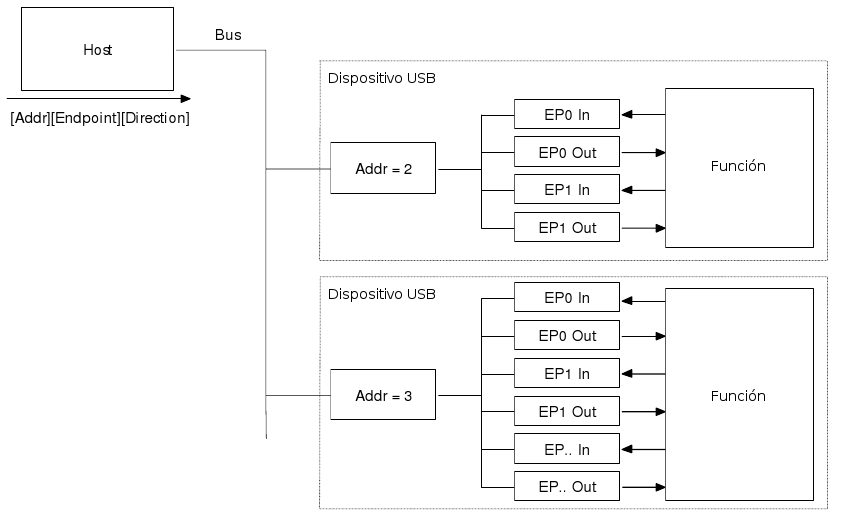
\includegraphics[scale=0.5]{./img/usb_endpoints.png}
\caption{Endpoints de USB.}
\label{fig:usb_endpoints}
\end{figure}

Entonces si por ejemplo el host emite un pedido de descripci\'on de dispositivo
(\emph{device descriptor request}) el dispositivo va a determinar por medio de
el campo \emph{ADDR} si el pedido esta dirigido hacia \'el, y luego copiar\'a
el dato en el endpoint correspondiente al que indica el campo \emph{ENDP}, que
luego podra ser leido por la aplicaci\'on embebida en el dispositivo.\\

El enpoint 0 debe existir en todos los dispositivos, ya cumple la funci\'on
espec\'ifica de realizar el handshaking y todo el control en una
comunicaci\'on USB. 


%%%%%%%%%%%%%%%%%%%%%%%%%%%%%%%%%%%%%%%%%%%%%%%%%%%%%%%%%%%%%%%%%%%%%%%%%%%%%%
%%%%%%%%%%%%%%%%%%%%%%%%%%%%%%%%%%%%%%%%%%%%%%%%%%%%%%%%%%%%%%%%%%%%%%%%%%%%%%
\section{Transferencias USB}
La especificaci\'on USB define cuatro tipos de transferencia:

\begin{itemize}
 \item Control
 \item Interrupt
 \item Isochronous 
 \item Bulk
\end{itemize}

Debido a el alcance de \'este trabajo solo se desarrollar\'an las
transferencias \emph{Control} y \emph{Bulk}, que fueron las usadas durante el
desarrollo del proyecto.


%%%%%%%%%%%%%%%%%%%%%%%%%%%%%%%%%%%%%%%%%%%%%%%%%%%%%%%%%%%%%%%%%%%%%%%%%%%%%%
\subsection{Control}
Las transferencias de control son usadas para petici\'on y reporte de estados o
emisi\'on de ordenes. Este tipo de transferencia posee tres etapas distintas:

\begin{itemize}
 \item Setup:
		Durante esta estapa se realiza la petici\'on de datos.
 \item Data:
		En esta etapa se realiza el intercambio de datos y puede consistir de
varias transferencias \emph{IN} o \emph{OUT} segun corresponda. 
 \item Status:
		Esta etapa se realiza al finalizar la transefrencia de control y
determina el exito o no de la operaci\'on.
\end{itemize}


%%%%%%%%%%%%%%%%%%%%%%%%%%%%%%%%%%%%%%%%%%%%%%%%%%%%%%%%%%%%%%%%%%%%%%%%%%%%%%
\subsection{Bulk}
Las transferencias tipo \emph{bulk}, son usadas para transmisi\'on de grandes
pedazos de datos. \'Este tipo transferencias provee correcci\'on de datos
con un campo \emph{CRC} de 16 bits y un mecanismo de detecci\'on y
re-trasmision de errores para asegurar la integridad de los mismos.\\

Las transferencias bulk no poseen un ancho de banda asignado, por lo cual no
aseguran latencia alguna.\\

Las transacciones bulk pueden ser de tipo \emph{IN} o \emph{OUT} como se ve en
la figura \ref{fig:usb_bulk_transaction}.

\begin{figure}
\centering
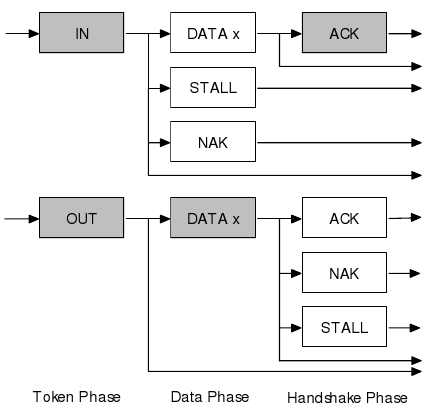
\includegraphics[scale=0.5]{./img/usb_bulk_transaction.png}
\caption{Transacci\'on Bulk.}
\label{fig:usb_bulk_transaction}
\end{figure}


%%%%%%%%%%%%%%%%%%%%%%%%%%%%%%%%%%%%%%%%%%%%%%%%%%%%%%%%%%%%%%%%%%%%%%%%%%%%%%
%%%%%%%%%%%%%%%%%%%%%%%%%%%%%%%%%%%%%%%%%%%%%%%%%%%%%%%%%%%%%%%%%%%%%%%%%%%%%%
\section{Descriptores USB}
% Revisar pagina 240 de la spec usb 2.0 grafico de estados para agregar
% Agregar proceso de enumeracion de la spec pag 243	
Los descriptores USB son estructuras de datos con formatos especif\'icos, en
los cuales se almacena todos los atributos del dispositivo.
Cada descriptor comienza con un campo donde se almacena el tama\~no de dicho
descriptor, seguido inmediatamente por un campo que identifica el tipo de
descriptor.\\
Entre los descriptotes mas comunes se enucentran:

\begin{itemize}
 \item Device: Cada dispositivo tiene un solo descriptor \emph{device}, y
\'estos poseen informaci\'on b\'asica sobre \'el. Entre otras cosas este
descriptor tiene un n\'umero identificador del vendedor y el dispositivo en
si. Tiene ademas un campo con la informacion de cuantas configuraciones
soporta el dispositivo.

 \item Configuration: Este descriptor posee entre otras cosas el tipo de
alimentaci\'on y el n\'umero de interfaces configuradas del dispositivo.

 \item Interface: Este descriptor puede ser visto como una cabecera con
informaci\'on sobre un grupo de endpoints.

 \item Enpoint: Este descriptor posee toda la informaci\'on necesaria para car
acterizar cada endpoint. Entre otras cosas aqui se define el tipo de
transefrencia que usa el endpoint (bulk, interrupt, isochronous, control), el
tama\~no de los paquetes, etc. El endpoint 0 siempre es cosiderado de control
y debe estar configurado.

 \item String: Estos descriptores poseen informaci\'on legible por humanos que
peden ser indexados por otros descriptores. 

\end{itemize}

Los desciptores pueden ser ordenados jer\'arquicamente segun se ve en la
figura \ref{fig:usb_descriptors}

\begin{figure}
\centering
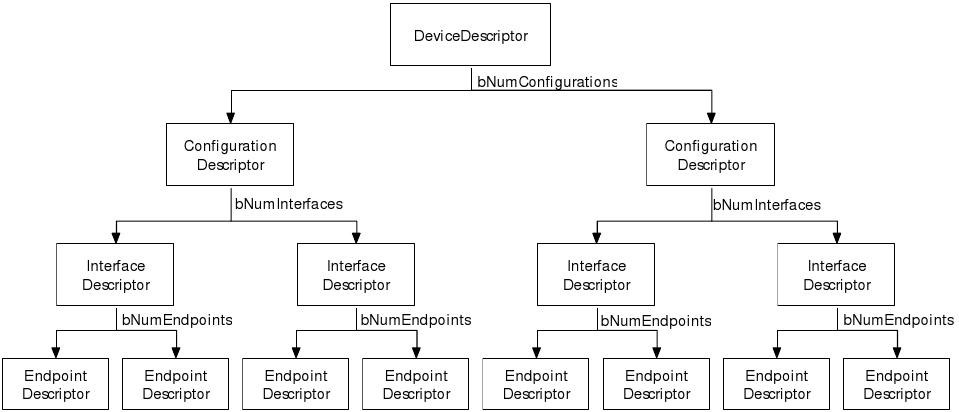
\includegraphics[scale=0.4]{./img/usb_descriptors.png}
\caption{Descriptores USB.}
\label{fig:usb_descriptors}
\end{figure}

%%%%%%%%%%%%%%%%%%%%%%%%%%%%%%%%%%%%%%%%%%%%%%%%%%%%%%%%%%%%%%%%%%%%%%%%%%%%%%
%%%%%%%%%%%%%%%%%%%%%%%%%%%%%%%%%%%%%%%%%%%%%%%%%%%%%%%%%%%%%%%%%%%%%%%%%%%%%%
\section{Estados USB}
Los dispositivos USB poseen varios estados definidos por los cuales pueden
transicionar durante su uso.
El diagrama de estados completo de un dispositivo USB puede verse en la figura
\ref{fig:usb_states}.


% Spec 2,.0 pag 240
\begin{figure}
\centering
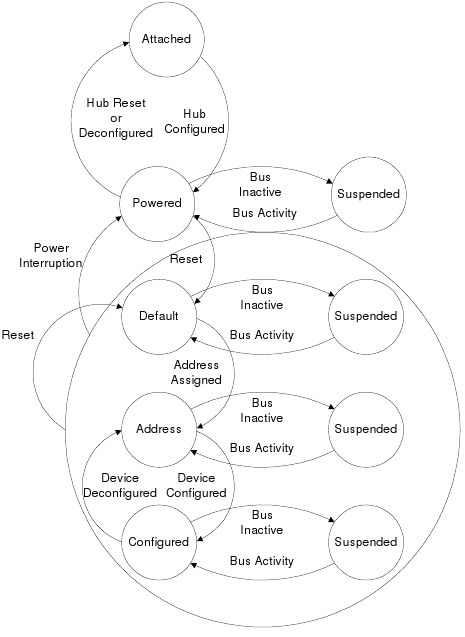
\includegraphics[scale=0.7]{./img/usb_states.png}
\caption{Estados USB.}
\label{fig:usb_states}
\end{figure}


En la tabla \ref{tab:usb_states}, se puede apreciar una breve explicaci\'on de
cada estado

% Spec 2,.0 pag 241
\begin{table}[h]
\begin{scriptsize}
\centering
\begin{tabular*}{\textwidth}{@{\extracolsep{\fill}}|c|c|c|c|c|c|p{5cm}|} \hline

% Header Titles
\rowcolor[gray]{.9}
Attached & Powered & Default & Address & Configured & Suspended
& Descripci\'on\\ \hline

% Table fill
% 1 %
No & -- & -- & -- & -- & -- & 
El dispositio no est\'a enchufado\\
\hline
% 2 %
Si & No & -- & -- & -- & -- & 
El dispositivo esta enchufado pero no alimentado.\\
\hline 
% 3 %
Si & Si & No & -- & -- & -- &
El dispositivo se encuentra enchufado y alimentado, pero no ha sido
reseteado.\\
\hline
% 4 %
Si & Si & Si & No & -- & -- &
El dispositico se encuentra enchufado, alimentado y ha sido reseteado, pero no
se le ha asignado una direcci\'on \'unica.\\
\hline
% 5 %
Si & Si & Si & Si & No & -- &
El dispositivo esta enchufado, alimentado, ha sido reseteado y se le ha
asignado una direcci\'on \'unica, pero no ha sigo configurado.\\
\hline
% 6 %
Si & Si & Si & Si & Si & No &
El dispositivo est\'a enchufado, alimentado, ha sido reseteado, se le ha
asignado una direcci\'on \'unica, ha sido configurado y no esta suspendido. El
host puede hacer uso del dispositivo ahora.\\
\hline
% 7 &
Si & Si & -- & -- & -- & Si &
El dispositivo se encuentra como minimo enchufado y alimentado, pero no ha
presentado actividad alguna en los ultimos 3 ms, por lo que el dipositivo se
encuentra suspendido y no puede ser usado por el host.\\
\hline 

\end{tabular*}
\caption{Estados USB.} 
\label{tab:usb_states}
\end{scriptsize}
\end{table}

%%%%%%%%%%%%%%%%%%%%%%%%%%%%%%%%%%%%%%%%%%%%%%%%%%%%%%%%%%%%%%%%%%%%%%%%%%%%%%
%%%%%%%%%%%%%%%%%%%%%%%%%%%%%%%%%%%%%%%%%%%%%%%%%%%%%%%%%%%%%%%%%%%%%%%%%%%%%%
\section{Enumeraci\'on del bus USB}
El proceso de enumeraci\'on determina si un dispositivo se ha conectado al
bus, a que puerto, sus configuraciones, intefaces, etc.
A continuaci\'on se listan los acciones que se llevan a cabo durante el
proceso de enumeraci\'on.

% Spec 2.0 pag 243
\begin{enumerate}
 % 1 %
 \item El hub a el cual el dispositivo esta conectado informa al host del
evento. En este paso el dispositivo se encuentra \emph{POWERED} y el puerto al
cual esta enchufado se encuentra deshabilitado.
 % 2 %
 \item El host determina la naturaleza del cambio consultandole al hub.
 % 3 %
 \item El host conoce ahora el puerto al cual se ha conectado el dispositivo y
espera 100 ms para que se normalice su alimentaci\'on. El host habilita el
puerto y envia una petici\'on de \emph{reset}.
 % 4 %
 \item El hub ejecuta el pedido de \emph{reset} para ese puerto y luego el
puerto queda habilitado. El dispositivo pasa a el estado \emph{DEFAULT} y no
puede consumir mas de 100 mA. Todos sus registros han sidos reseteados y
responde a la direcci\'on por defecto.
 % 5 %
 \item El host asigna una direcci\'on \'unica al dispositiv y esta pasa al
estado \emph{ADDRESS}.
 % 6 %
 \item El host lee del dispositivo el tama\~no de datos que puede recibir antes
de que \'este reciba la direcci\'on.
 % 7 %
 \item El host lee toda la configuracion de dispositivo.
 % 8 %
 \item Basado en la configuraci\'on obtenida, el host asigna un valor de
configuraci\'on al dipositivo y \'este pasa a el estado de \emph{CONFIGURED}.
Desde el puento de vista del dipositivo \'este se encuentra listo para ser
usado.
\end{enumerate}

%%%%%%%%%%%%%%%%%%%%%%%%%%%%%%%%%%%%%%%%%%%%%%%%%%%%%%%%%%%%%%%%%%%%%%%%%%%%%%
%%%%%%%%%%%%%%%%%%%%%%%%%%%%%%%%%%%%%%%%%%%%%%%%%%%%%%%%%%%%%%%%%%%%%%%%%%%%%%
\section{PIC18F4550 USB}
% Habra que ponerle el cosito de copyright al lado de Microchip?
La familia de microcontroladores PIC18FX455/X550 de Microchip provee
conexi\'on USB de tipo \emph{full} y \emph{high-speed}. Dicha comunicaci\'on
se lleva acabo mediante lo que Microchip denomina \emph{USB Serial Interface
Engine} (\emph{USB SIE}) o simplemente \emph{SIE}. 
El \emph{SIE} es capaz de interactuar con un transceptor tanto externo como
con interno. Y se provee tambien un regulador de voltaje de 3.3V interno
completamente integrado para alimentar el tranceptor.

En la figura \ref{fig:pic_usb_internal} se muestra un diagrama interno de
la arquitectura USB de \'esta familia de microcontroladores.

% Datasheet pag 163
\begin{figure}
\centering
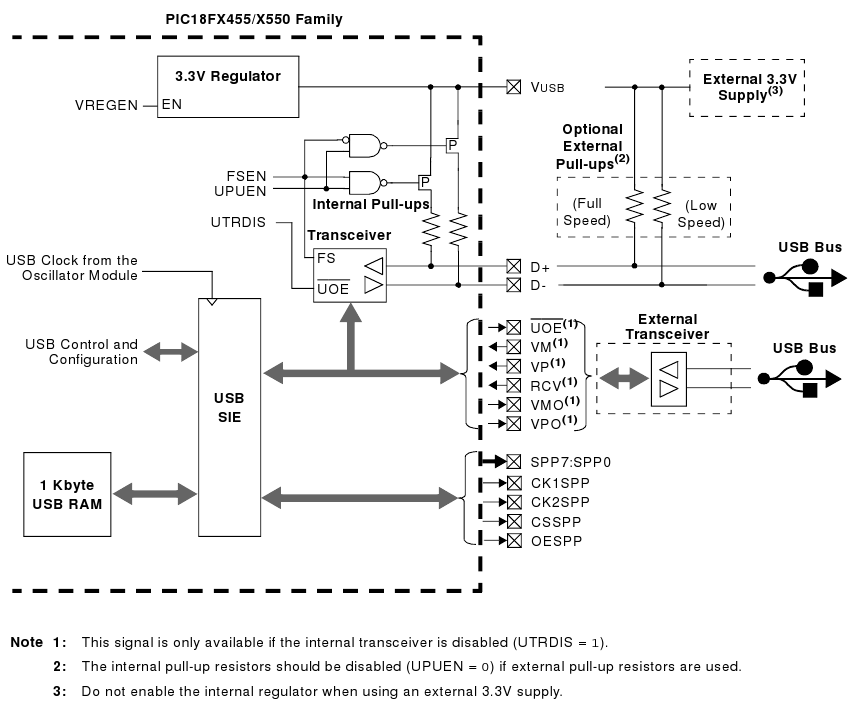
\includegraphics[scale=0.5]{./img/pic_usb_internal.png}
\caption{Arquitectura USB de la familia PIC18FX455/X550.}
\label{fig:pic_usb_internal}
\end{figure}


\subsection{Registros}
El modulo USB es controlado mediante 22 registros diponibles en el
microcontrolador, la mayoria de los cuales son de lectura y escritura.




%%%%%%%%%%%%%%%%%%%%%%%%%%%%%%%%%%%%%%%%%%%%%%%%%%%%%%%%%%%%%%%%%%%%%%%%%%%%%%
%%%%%%%%%%%%%%%%%%%%%%%%%%%%%%%%%%%%%%%%%%%%%%%%%%%%%%%%%%%%%%%%%%%%%%%%%%%%%%
\section{USB en linux}

Linux comenz\'o a soportar el protocolo USB desde la versi\'on 2.2.7
(\emph{principio de 1999}), con codigo aportado por el mismo \emph{Linus
Torvalds\footnote{Codigo fuente
en: ftp://ftp.kernel.org/pub/linux/kernel/testing/old/usb/}
\footnote{V\'ease:
http://marc.info/?l=linux-usb\&m=92282561930486\&w=2}
}.\\

Con el paso del tiempo el soporte de linux para el protoco USB ha aumentado
considerablemente, y actualmente existen drivers para una enorme cantidad de
dispositivos.\\

Linux interpone varias capas de abstracci\'on entre el usuario y el hardware
USB, en la figura \ref{fig:usb_linux_layers} se puede apreciar una
representacion de dichas capas.

\begin{figure}
\centering
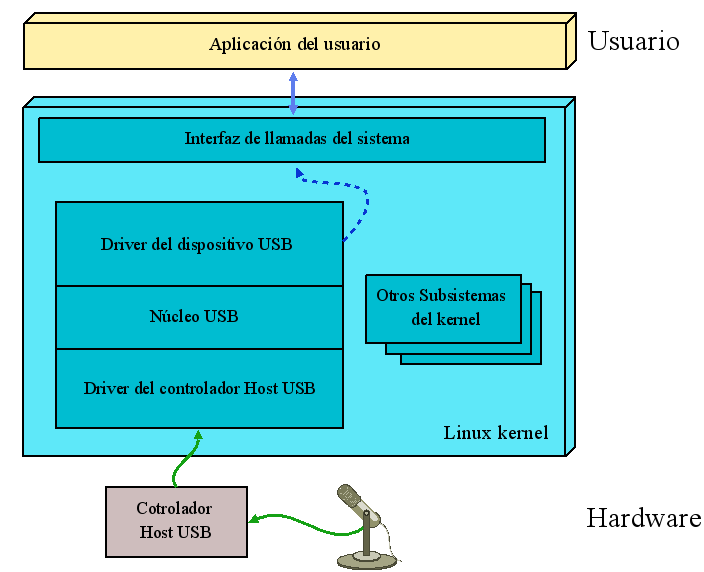
\includegraphics[scale=0.5]{./img/usb_linux_layers.png}
\caption{Soporte USB de linux.}
\label{fig:usb_linux_layers}
\end{figure}


En los cap\'itulos siguientes se describir\'a como es manejado el protocolo a
nivel del kernel y una \emph{API} libre de mas alto nivel.


%%%%%%%%%%%%%%%%%%%%%%%%%%%%%%%%%%%%%%%%%%%%%%%%%%%%%%%%%%%%%%%%%%%%%%%%%%%%%%
\subsection{Manejo USB de bajo nivel}

El kernel linux posee documentaci\'on embebida, la cual puede ser generada en
formato \emph{postscipt} \footnote{V\'ease -
http://es.wikipedia.org/wiki/PostScript}, pdf, o html. Para lograr esto basta
con bajar el codigo del kernel y compilar la documentaci\'on de la siguiente
manera:

\begin{scriptsize}
	\begin{verbatim}
	$ wget http://www.kernel.org/pub/linux/kernel/v2.6/linux-x.y.z.tar.bz2
	$ tar -xjf linux-x.y.z.tar.bz2
	$ cd  linux-x.y.z/
	$ make pdfdocs
	\end{verbatim}
\end{scriptsize}

En la documentaci\'on generada se encuentra una secci\'on espec\'ifica sobre
USB.\\

Basicamente linux posee en su nivel m\'as bajo drivers para el controlador
host (ya sean UHCI, OHCI o EHCI), el cual se comunica con el
\emph{usbcore}\footnote{Tambi\'en llamado API, pero aqui nos referiremos como
\emph{usbcore} o \emph{core} por cuestiones pr\'acticas.} quien interactua
directamente con los drivers espec\'ificos de cada dispositivo (Ver figura
\ref{fig:usb_linux_layers}).


%% Esto ya no es tan bajo nivel, deberi tener otra seccion
En el c\'odigo fuente del kernel existe un \emph{esquelto}\footnote{V\'ease
- http://lxr.linux.no/linux+v2.6.28/drivers/usb/usb-skeleton.c} de un driver
gen\'erico, con varias variables definidas, funciones y macros \'utiles.
Este \emph{esqueleto} fue escrito por Greg Kroah-Hartman\footnote{Mail - 
greg@kroah.com} y basado en \emph{pci-skeleton.c}\footnote{V\'ease -
http://lxr.linux.no/linux+v2.6.28/drivers/net/pci-skeleton.c}.
Este \emph{driver gen\'erico} posee todo lo necesario para , con
modificaciones suficientes, escribir un driver espec\'ifico de un dispositivo.


%%%%%%%%%%%%%%%%%%%%%%%%%%%%%%%%%%%%%%%%%%%%%%%%%%%%%%%%%%%%%%%%%%%%%%%%%%%%%%
\subsection{URBs (API de bajo nivel)}

El kernel maneja\footnote{Si bien es la forma mas recomendada, puede evitarse
el uso de esta API} el acceso de los distintos drivers al sistema USB mediante
mensajes de \emph{pedidos de bloques USB} (\emph{URB - USB Request
Block}\footnote{El acronimo \emph{URB} se usar\'a en el documento por
cuestiones pr\'acticas}).\\

El concepto b\'asico de \emph{URBs} es el paso de mensajes de forma
asincr\'onica. 
Un \emph{URB} contine toda la informacion necesaria para hacer una
transacci\'on USB y provee ademas un \emph{manejador}\footnote{\emph{Handler}
en ingles.} con toda la informaci\'on de la transacci\'on.
Por la naturaleza as\'incrona de los URBs, ni bien se env\'ian, estos son
encolados y la funci\'on vuelve inmediatamente. 

% FAAAAKKKKK como mierda me las arreglo para explicar todo esto, que
% quilombo!!!!
% Seguir...


%%%%%%%%%%%%%%%%%%%%%%%%%%%%%%%%%%%%%%%%%%%%%%%%%%%%%%%%%%%%%%%%%%%%%%%%%%%%%%
\subsection{API de alto nivel - libusb}

La API \emph{libusb} consiste en un set de librerias de codigo abierto
licenciadas bajo LGPL (%Expandir el nombre y poner footnote con url
% Hacer lo mismo con libusb ). 
Dichas librerias resuelven la comunicaci\'on
USB pero a nivel de usuario.
La API se encuentra en casi todoas las distribuciones de GNU/Linux, y se
presenta en forma de libreria dinamica para usar con aplicaciones ya
compiladas y un paquete extra para \emph{development}\footnote{Del ingles
desarrollo}, con los archivos cabecera, programas para compilar, y
la documentaci\'on completa de sus funcionalidades con algunos ejemplos
extras. \\

La libreria provee entre definiciones y estructuras, las siguientes funciones:



\begin{lstlisting}
/* usb.c */
usb_dev_handle *usb_open(struct usb_device *dev);
int usb_close(usb_dev_handle *dev);
int usb_get_string(usb_dev_handle *dev, int index, int langid, char *buf,
size_t buflen);
int usb_get_string_simple(usb_dev_handle *dev, int index, char *buf,size_t
buflen);

/* descriptors.c */
int usb_get_descriptor_by_endpoint(usb_dev_handle *udev, int ep, unsigned char
type, unsigned char index, void *buf, int size);
int usb_get_descriptor(usb_dev_handle *udev, unsigned char type, unsigned char
index, void *buf, int size);

/* <arch>.c */
int usb_bulk_write(usb_dev_handle *dev, int ep, const char *bytes, int size,
int timeout);
int usb_bulk_read(usb_dev_handle *dev, int ep, char *bytes, int size, int
timeout);
int usb_interrupt_write(usb_dev_handle *dev, int ep, const char *bytes,
int size, int timeout);
int usb_interrupt_read(usb_dev_handle *dev, int ep, char *bytes, int size, int
timeout);
int usb_control_msg(usb_dev_handle *dev, int requesttype, int request, int
value, int index, char *bytes, int size, int timeout);
int usb_set_configuration(usb_dev_handle *dev, int configuration);
int usb_claim_interface(usb_dev_handle *dev, int interface);
int usb_release_interface(usb_dev_handle *dev, int interface);
int usb_set_altinterface(usb_dev_handle *dev, int alternate);
int usb_resetep(usb_dev_handle *dev, unsigned int ep);
int usb_clear_halt(usb_dev_handle *dev, unsigned int ep);
int usb_reset(usb_dev_handle *dev);
\end{lstlisting}


Todas las funciones de esta libreria (para la version estable 0.1) son
s\'incronas, lo que significa que se debe esperar a que termine la operaci\'on
para poder seguir. Por este motivo la mayoria de las funciones implemetan un
\emph{timeout} en milisegundos.\\

% Poner primero, antes del codigo, un diagrama de flujo del mismo


Para comenzar una comunicaci\'on USB con esta libreria es preciso primero
descubrir el dipositivo, esto se logra con:

\begin{lstlisting}
struct usb_bus *busses;
    
usb_init();
usb_find_busses();
usb_find_devices();
    
busses = usb_get_busses();
\end{lstlisting}

Luego de esto ya se poseen los \emph{busses} USB del sitema. Es preciso luego
iterar sobre cada uno de ellos para encontrar el dispositivo especifico de la
siguiente manera:

\begin{lstlisting}
struct usb_bus *bus;
int c, i, a;
    
/* ... */
    
for (bus = busses; bus; bus = bus->next) {
  struct usb_device *dev;
    
    for (dev = bus->devices; dev; dev = dev->next) {
        /* Buscar el dispositivo por VendorID */
        if (dev->descriptor.idVendor == MY_ID) {
            /* Buscar el dispositivo por ProductID */
            if (dev->descriptor.idProduct==USBPRINTER){
            /* Abrir dispositivo */
            udev = usb_open(dev);
            /* Reclamar la interfaz */
            ret = usb_claim_interface(udev,0); 

            /* Programa */
            }	...
        }
    }
}
\end{lstlisting}

Una limitaci\'on intr\'inseca de la libreria es que se requiere abrir tantas
instancias del dispositivo como interfaces se desee usar de \'el.\\

Estas librerias satisfacen tanto el estandar USB 1.0 como el 2.0, es por ello
que si el dispositivo respeta el estandar, establecer una comunicaci\'on a
USB requiere solo la adici\'on de algunas funciones al codigo fuente para;
inicializar la comunicaci\'on, para buscar el dispositivo, para abrirlo y
luego el programa en si.


% Requerido por reglamento de trabajo final 
\chapter{Diagn\'ostico}

% Aca va una descripcion y analisis del problema abordado, un breve contenido
% de fundamento social y planteo de las necesidades.
% Incluir las razones qeu motivan este trabajo y se puede incluir una breve
% aproximacion historica.

% es recomendable dejarlo casi al final del trabajo

% Diagnóstico, en el mismo se mostrará la problemática actual, las
% dificultades a superar y todo aquello que se considere de interés y
% necesario para comprender el propósito que nos impulsa a tratar el tema.

En la actualidad existen muchas empresas que fabrican dispositivos de
impresi\'on braille, pero debido a el tama\~no reducido del nicho de mercado
en el que se encuentran, sus precios suelen ser muy elevados y no est\'an al
alcance del ciudadano medio.\ Y al pertenecer, de una forma u otra, a un sector
tecnol\'ogico, existe una gran competencia en cuanto al avance de sus
tecnolog\'ias. Esto conlleva a que fabriquen dispositivos con muchas
funcionalidades, prestaciones y de gran performance, dejando de lado dise\~nos
sencillos y meramente funcionales que har\'ian al producto menos costoso.\\

Otro problema que presentan estos dispositivos, es que, a falta de est\'andares
de impresi\'on braille, cada fabricante provee su propia soluci\'on de
software que suele ser un costo extra en algunas ocasiones.\ 
Por este mismo motivo el soporte que proveen suele limitarse a un \'unico
sistema operativo\footnote{Normalmente Microsoft Windows.} forzando al usuario
a comprar una licencia del mismo e incluso en muchos casos un \'unico
procesador de texto\footnote{Normalmente Word de la suite Microsoft Office.}.\\

Se encuentra tambi\'en dicha industria embebida en modelos de desarrollo
privativo, haciendo imposible al usuario final a agregar sus propios cambios
bas\'andose en sus necesidades particulares.\ Si bien el modelo de desarrollo
privativo es uno de los mas usados en todas las industrias, existen varias que
se encuentran, ya sea en etapas de exploraci\'on o producci\'on, trabajando con
modelos \emph{C\'odigo Abierto}\footnote{Del ingl\'es \emph{open-source}} o
incluso \emph{Software Libre}\footnote{Del ingl\'es \emph{ Free Software}},
siendo esto un lujo que la industria de dispositivos de impresi\'on braille no
puede darse debido mayormente a su tama\~no.\\

Las problem\'aticas antes planteadas hacen que un posible mercado nacional de
estas tecnolog\'ias sea pr\'acticamente imposible, por lo que las impresoras
braille deben ser adquiridas en el exterior o mediante un importador.\\

% Todo esto ###### <---buscar una palabra mejor
Todo esto termina en que los usuarios finales deben gastar una importante suma
de dinero para poder realizar impresiones braille en su hogar, comprando un
sistema operativo, una suite ofim\'atica, y un dispositivo con prestaciones
que exceden las necesidades del mismo.


% ----------------------------------------------------------------------------

\end{document}
